\documentclass[]{article}
\usepackage{amsmath, amssymb, graphicx, float, dsfont}

%opening
\title{Notes on Least Squares Optimization}
\author{Delbert Yip}

\newcommand{\norm}[1]{\lvert #1 \rvert}

\begin{document}

\maketitle

\begin{abstract}
	These notes were taken from Chapter 8 from Strang's "Computational Science and Engineering," \cite{strang_computational_2012} and cover ordinary, weighted, and regularized least squares (Sections 8.1-8.3 of \cite{strang_computational_2012}). Some background material has been taken from Lay's "Linear algebra and its applications" \cite{lay_linear_2012}.
\end{abstract}

\section{Least Squares}
Consider a matrix A of size $m x n$ with $n$ independent columns, and $m > n$. 
$A^T A$ is symmetric positive definite, as Rank(A) = $n$. 
We wish to solve $Au = b$ for some vector $b$ with $m$ components. The solution $\hat{u}$ has $n$ components. 

This gives rise to the \textbf{least squares problem}:
\begin{equation}
\min \parallel Au - b \parallel ^2 
\end{equation}

Below are the normal equations, which give the solution $\hat{u}$:
\begin{align} 
Au &= b \nonumber \\
A^T A \hat{u} &= A^T b 
\end{align}

The residual of the cost function is $e = b - Au$, and has dimensions $m \times 1$. Thus, 
\begin{equation}
A^T e = A^T b - A^T A u
\end{equation}
Therefore, $A^T e = 0$ when $u = \hat{u}$. 

$e$ is in the nullspace of $A^T$, and is therefore perpendicular to the columns (column space) of $A$ (equivalently, $e$ is perpendicular to the rows/rowspace of $A^T$). Recall that orthogonality means that the dot product of two vectors is 0. 

\subsection{Refresher on Orthogonality}
Before we start on the next section, let's review some concepts from linear algebra. Specifically, the orthogonality of vectors and vector spaces. 

 Orthogonal Vectors 
There is an analogue between geometry in Euclidean space and in $\mathds{R}^n$. 

First, *two vectors $\mathbf{u}$ and $\mathbf{v}$ are perpendicular i.f.f. the distance between $\mathbf{u}$ and $\mathbf{-v}$ is the same as the distance between $\mathbf{u}$ and $\mathbf{+v}$.* 

First, the distance between $\mathbf{u}$ and $\mathbf{-v}$:
\begin{align}
[\textrm{dist}(\mathbf{u}, \mathbf{-v})]^2 &= \parallel \mathbf{u}-(-\mathbf{v}) \parallel ^2 = \parallel \mathbf{u} +\mathbf{v} \parallel ^2 \\
&= (\mathbf{u} + \mathbf{v}) \cdot (\mathbf{u} + \mathbf{v}) \\ 
&= \parallel \mathbf{u} \parallel^2 + \parallel \mathbf{v} \parallel^2 + 2\mathbf{u} \cdot \mathbf{v}
\end{align}

Next, the distance between $\mathbf{u}$ and $\mathbf{+v}$:
\begin{align}
[\textrm{dist}(\mathbf{u}, \mathbf{v})]^2 &= \parallel \mathbf{u} -\mathbf{v} \parallel ^2 \\
&= (\mathbf{u} - \mathbf{v}) \cdot (\mathbf{u} - \mathbf{v}) \\ 
&= \parallel \mathbf{u} \parallel^2 + \parallel \mathbf{v} \parallel^2 - 2\mathbf{u} \cdot \mathbf{v}
\end{align}

Therefore, 

\begin{align}
	[\textrm{dist}(\mathbf{u}, \mathbf{-v})]^2 = [\textrm{dist}(\mathbf{u}, \mathbf{v})]^2 &\iff - 2\mathbf{u} \cdot \mathbf{v} = 2\mathbf{u} \cdot \mathbf{v} \\
	&\implies \quad \mathbf{u} \cdot \mathbf{v} = 0 \\
	&\implies \parallel \mathbf{u} + \mathbf{v} \parallel ^2 = \parallel \mathbf{u} \parallel^2 + \parallel \mathbf{v} \parallel^2
\end{align}

\subsection{Orthogonal Complements in $\mathds{R}^n$}
If a vector $\mathbf{z}$ is orthogonal to every vector in a subspace $W$ of $\mathds{R}^n$, then $\mathbf{z}$ is orthogonal to $W$. The set of all such vectors $\mathbf{z}$ is the \textbf{orthogonal complement} of $W$ and denoted by $W^\bot$. Let's go through the relation between nullspace, orthogonal complements, and the columns and rows of a $m \times n$ matrix $A$. 

We have the folllowing theorem: 
\begin{equation}
(\textrm{Row}(A))^\bot = \textrm{Nul}(A) \quad \textrm{and} \quad (\textrm{Col}(A))^\bot = \textrm{Nul}(A)^\bot 
\end{equation}

If $Ax = 0$ for some $n \times 1$ vector $x$, then $x \in \textrm{Nul}(A)$, which means $x$ is orthogonal to the rows of $A$. The rows of $A$ span its row space, so $x$ is orthogonal to Row($A$). This is a consequence of how matrix multiplication works, as shown below: 
\begin{align}
	A &= \begin{pmatrix} a & b & c \\ d & e & f \end{pmatrix}, \quad u = \begin{pmatrix} x \\ y \\ z \end{pmatrix}. \\
	Au &= \begin{pmatrix}	a \\ d	\end{pmatrix} x + \begin{pmatrix}	b \\ e	\end{pmatrix} y + \begin{pmatrix}	c \\ f	\end{pmatrix} z, \quad \textrm{ linear combination of the columns}\\
		&= \begin{pmatrix} ax + by + cz \\ dx + ey + fz \end{pmatrix}, \quad \textrm{ dot product of the rows}\\
		&= \begin{pmatrix} 0 \\ 0 \end{pmatrix} 
\end{align}

The elements of the product $Au$ are dot products between $u$ and the row vectors of $A$; the product $Au$ can also be thought of as a linear combination of the columns of $A$. Since $Au = 0$, $u$ is in the nullspace of A, and from the above, we see that $u$ is orthogonal to the rows of $A$.

\begin{figure}[H]
	\centering
	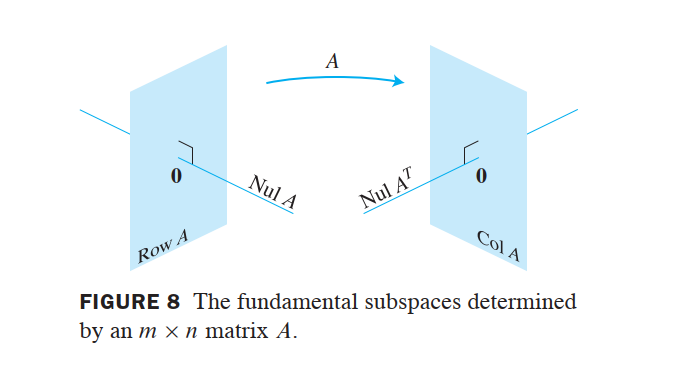
\includegraphics[width=0.7\linewidth]{figs/Lay_fundamental_subspaces}
	\caption{Fundamental subspaces of $A$. From Lay.}
	\label{fig:layfundamentalsubspaces}
\end{figure}


\subsection{Primal and Dual Problems}
In the 'primal' problem, we find the solution $\hat{u}$ by projecting $b$ onto the column space of $A$, i.e. $A\hat{u}$ is the closest point to $b$ in the column space of $A$. In general, the product $Au$ yields a linear combination of the columns of $A$. The column space of $A$ contains all such products. 

\begin{equation}
Au = y \quad \implies \quad y \in \textrm{Col}(A), \quad \forall u
\end{equation}
Where, Col($A$) refers to the column space of $A$. 

The 'dual' problem solves $A^T e = 0$ for $e$, which is the projection of $b$ onto the nullspace of $A^T$. Recall from above: 
$$ \textrm{Nul}(A^T) = (\textrm{Row}(A^T))^\bot = (\textrm{Col}(A))^\bot $$
Thus, $e$ is contained in (Col($A$))$^\bot$, which contains \textit{all vectors perpendicular to the columns of $A$}. The dimension of (Col($A$))$^\bot$ is given by the Rank-Nullity Theorem: 

\begin{align}
	&\textrm{Rank}(A) + \textrm{Nullity}(A) = n, \quad \textrm{ where } n \textrm{ is the number of columns in } A. \\
	&\textrm{Rank}(A^T) + \textrm{Nullity}(A^T) = m \\ 
	&\textrm{Rank}(A) = \textrm{Rank}(A^T) \quad \implies \quad \textrm{Nullity}(A^T) = m - n \\
	&\textrm{Nullity}(A^T) = \textrm{dim(Row(}A^T))^\bot = \textrm{dim(Col(}A)^\bot) = m - n
\end{align}

\begin{figure}[H]
	\centering
	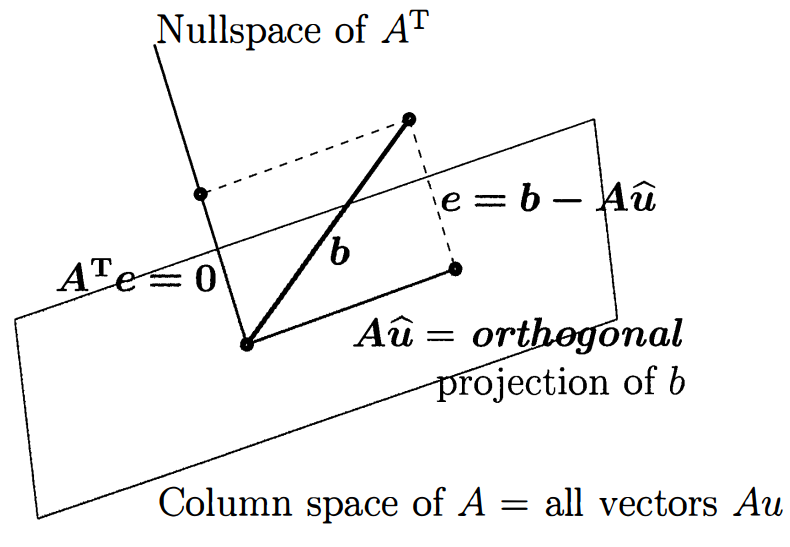
\includegraphics[width=0.7\linewidth]{figs/Strang_projection_lsq}
	\caption{Ordinary least squares. From Strang.}
	\label{fig:strangprojectionlsq}
\end{figure}

$e$ and $\hat{u}$ solve the two linear equations shown by the figure above:
\begin{align}
e + A \hat{u} &= b \rightarrow m \textrm{ equations} \\
A^T e &= 0 \rightarrow n \textrm{ equations}
\end{align}

These are called the "Primal-Dual", "Saddle Point", and "Kuhn-Tucker (KKT)" equations. 

\subsubsection{"Saddle Point" Equations}
The Saddle Point, or KKT, matrix is a block matrix that represents the Primal-Dual equations:
$$ S = \begin{bmatrix} I & A \\ A^T & 0 \end{bmatrix} \quad \implies \quad S \begin{bmatrix} e \\ \hat{u} \end{bmatrix} = \begin{bmatrix} Ie + A\hat{u} \\ A^T e + 0 \end{bmatrix} $$ 
Where, $I$ is an $m \times m$ identity matrix. Thus, $I$ constitutes the first $m$ pivot columns of $S$. Thus, to reduce $S$, we need to make the lower left hand corner of $S$ a $n \times n$ matrix of zeroes. To do this, let's review elimination on block matrices: 

\textbf{Elimination of block matrices}: 

\begin{align}
\begin{bmatrix} I & 0 \\ -CA^{-1} & I \end{bmatrix} \begin{bmatrix} A & B \\ C & D \end{bmatrix} &= \begin{bmatrix} A + 0 & B + 0 \\ -CA^{-1}A + C & -CA^{-1}B + D \end{bmatrix} \\
&= \begin{bmatrix} A & B \\ 0 & D - CA^{-1}B \end{bmatrix} 
\end{align}

The first matrix, $\begin{bmatrix} I & 0 \\ -CA^{-1} & I \end{bmatrix}$, is also known as the Gaussian elimination matrix, often represented using the symbol $E$. If $A$ was not an identity matrix, then we can also reduce $A$ into a matrix of pivots: 

\begin{align}
\begin{bmatrix} A^{-1} & 0 \\ -CA^{-1} & I \end{bmatrix} \begin{bmatrix} A & B \\ C & D \end{bmatrix} &= \begin{bmatrix} AA^{-1} + 0 & BA^{-1} + 0 \\ -CA^{-1}A + C & -CA^{-1}B + D \end{bmatrix} \\
&= \begin{bmatrix} I & BA^{-1} \\ 0 & D - CA^{-1}B \end{bmatrix} 
\end{align}


We now reduce our Primal-Dual matrix $S$ with $E = \begin{bmatrix} I & 0 \\ -A^T & I \end{bmatrix}$:

\begin{align}
ES &= \begin{bmatrix} I & 0 \\ -A^T & I \end{bmatrix} \begin{bmatrix} I & A \\ A^T & 0 \end{bmatrix} \\
	&= \begin{bmatrix} I + 0 & A + 0 \\ -A^T + A^T & -AA^T + 0 \end{bmatrix} \\
	&= \begin{bmatrix} I & A \\ 0 & -AA^T \end{bmatrix}
\end{align}

By convention, the lower right-hand block remaining after elimination is known as the \textbf{Schur complement}. More importantly, the first $m$ pivots are positive (=1), but the final $n$ pivots, determined by $-AA^T$, are negative. When a matrix has pivots of both signs, it is \textbf{indefinite}. For such matrices, \textit{there is no maximum or minimum, positive or negative definite}. Instead, there is a \textbf{saddle point, $(\hat{u}, e)$}.

\subsubsection{"Primal-Dual" Equations}
The \textit{primal} problem is to minimize $\frac{1}{2} \parallel Au - b \parallel^2$. The \textit{dual} problem is to minimize $\frac{1}{2} \parallel e - b \parallel^2$ with the constraint $A^T e = 0$. In the dual problem, $u$ acts a Lagrange multiplier to enforce the constraint $A^T e = 0$. Solutions to the primal and dual problems are found simultaneously, and add to $b$. 

Let's do an example!

\subsubsection{An Example}
\begin{equation}
A = \begin{bmatrix}2 \\ 1 \end{bmatrix}, \quad b = \begin{bmatrix}3 \\ 4\end{bmatrix}, \quad A^T A = 5, \quad A^T b = 10 
\end{equation}
\begin{align}
	&\textrm{Projection: } A\hat{u} = \begin{bmatrix}4 \\ 2\end{bmatrix} \\ 
	&\textrm{Error: } e = b - A\hat{u} = \begin{bmatrix}3 \\ 4 \end{bmatrix} - \begin{bmatrix}4 \\ 2\end{bmatrix} = \begin{bmatrix}-1 \\ 2\end{bmatrix} 
\end{align}

Let's verify that $A\hat{u}$ and $e$ are perpendicular. First, $A\hat{u}$ and $e$ sum to $b$:

\begin{equation}
A\hat{u} + e = A\hat{u} + (b - A\hat{u}) = b
\end{equation}

\begin{align}
\parallel b \parallel^2 &= \parallel A\hat{u} \parallel^2 + \parallel e \parallel^2 \\
&= 20 + 5 = 25 \\
A \hat{u} \cdot e &= \parallel A \hat{u} \parallel \parallel e \parallel \cos \theta \\
0 &= \sqrt{20} \sqrt{5} \cos \theta \\
\therefore \cos \theta &= 0 \quad \implies \quad \theta = \frac{\pi}{2} 
\end{align}

The normal equation is: $A^T A \hat{u} = A^T b$, so $\hat{u} = 2$. This solves the primal problem. The dual minimizes $\frac{1}{2}\parallel e-b \parallel^2$ under the constraint $A^T e = 0$. The solution to the dual problem gives $e$ and $\hat{u}$:

The \textbf{Lagrange} function is:

\begin{align}
L &= \frac{1}{2}\parallel e-b \parallel^2 + u(A^T e) \\
L(e_1, e_2, u) &= \frac{1}{2}(e_1 - b_1 )^2 + \frac{1}{2}(e_2 - b_2 )^2 + u(A^{T}_{1} e_1 + A^{T}_{2} e_2) \\
\frac{\partial L}{\partial (e_1, e_2, u)} &= \begin{bmatrix}
	e_1 - b_1 + 2\hat{u} = 0 \\
	e_2 - b_2 + \hat{u} = 0 \\
	2e_1 + e_2 = 0 
\end{bmatrix} = \begin{bmatrix}
	e_1 & e_2 & \hat{u} \\
	1 & 0 & 2 \\
	0 & 1 & 1 \\
	2 & 1 & 0 
\end{bmatrix} \begin{bmatrix} e_1 \\ e_2 \\ \hat{u} \end{bmatrix} = \begin{bmatrix} b_1 \\ b_2 \\ 0 \end{bmatrix}
\end{align}

The matrix $
\begin{bmatrix}
1 & 0 & 2 \\
0 & 1 & 1 \\
2 & 1 & 0 
\end{bmatrix} $
is the saddle point matrix $S$, whose columns correspond to $e_1$, $e_2$, and $u$, respectively. 

\section{Weighted Least Squares} \label{Weighted Least Squares}
The weighted least squares equation is:
\begin{equation}
\min \parallel WAu - Wb \parallel^2 
\end{equation}

with normal equations:
\begin{align}
(WA)^T (WA) \hat{u}_W &= (WA)^T (Wb) \\
A^T W^T W A \hat{u}_W &= A^T W^T W b \\
A^T C A \hat{u}_W &= A^T C b, \quad C = W^T W \\
\implies 0 &= A^T C b - A^T C A \hat{u}_W \\
	&= A^T C (b - A \hat{u}_W ) = A^T C e, \quad e = (b - A \hat{u}_W )
\end{align}

Where, $\hat{u}_W$ is the solution, and changes with the weight matrix $W$. Let's consider the geometric effects of introducing $W$. 
\begin{itemize}
	\item First, $A^T e = 0$ becomes $A^T C e = 0$. So, $e$ is perpendicular to $A^T C$ now, not $A^T$ by itself. So, $e$ is in the nullspace of $A^T C$, not that of $A^T$.
	\item With $W$, $e$ is now in the orthogonal complement to the rows of $A^T C$, or equivalently, the columns of $C^T A$. Thus, $e$ is not orthogonal to the column space of $A$. We say that $e$ is "$C$-orthogonal" to the columns of $A$. 
	\item Consequently, solving weighted least squares involves finding a projection of $b$ that is orthogonal to Col($C^T A)$, but not Col($A$).
	\item We still split $b$ into two components: $A\hat{u}_W \in \textrm{Col}(A)$, and $e \in \textrm{Nul}(A^T C)$.
\end{itemize}

\begin{figure}[H]
	\centering
	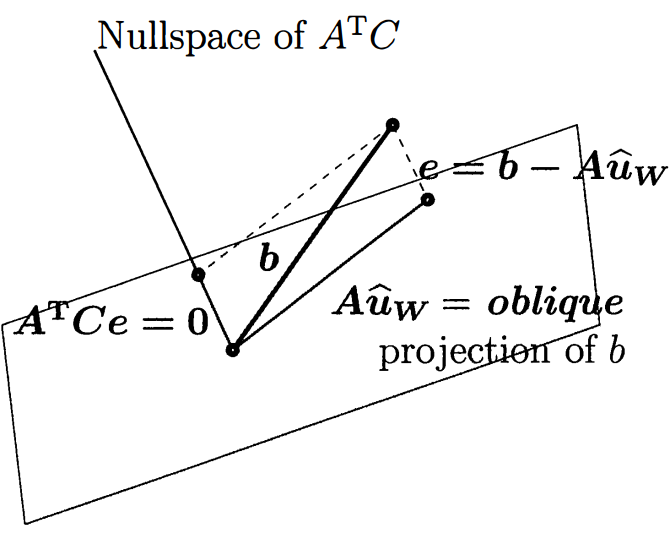
\includegraphics[width=0.7\linewidth]{figs/Strang_projection_wlsq}
	\caption{Weighted least squares.}
	\label{fig:strangprojectionwlsq}
\end{figure}


So, we have the following primal-dual equations to solve:
\begin{align}
e + A \hat{u}_W &= b \\ 
A^T C e &= 0 
\end{align}

The saddle point matrix is: \begin{equation}
\begin{bmatrix}
	I & A \\
	A^T C & 0
\end{bmatrix}, 
\end{equation} where the columns represent coefficients of $e$ and $\hat{u}_W$, respectively. Ideally, we'd like that the equations be symmetric. However, we have a factor of $C$ in the bottom-left that is not in the top-right, so our current matrix is not symmetric. To make it symmtric, introduce $w = Ce$ and $e = C^{-1}w$, and let $\hat{u}_W = u$:

\begin{align}
C^{-1}w + Au &= b \label{wlsq1} \\
A^T w &= 0 \label{wlsq2}
\end{align}

This gives rise to a symmetric matrix: \begin{equation}
S = \begin{bmatrix}
	C^{-1} & A \\ A^T & 0
\end{bmatrix},
\end{equation} where columns represent coefficients for $w$ and $u$, respectively. Since $C = W^T W$, which is the vector analogue to squaring, the elements of $C$, and thus $C^{-1}$, are positive. $W$ is a $m \times n$ matrix, so $C^{-1}$ contributes $m$ \textit{positive} pivot columns. The remaining pivots are found by elimination on $S$:

\begin{align}
E &= \begin{bmatrix} I & 0 \\ -A^T C & I  \end{bmatrix} \\
ES &= \begin{bmatrix} I & 0 \\ -A^T C & I  \end{bmatrix} \begin{bmatrix} C^{-1} & A \\ A^T & 0 \end{bmatrix} \\
	&= \begin{bmatrix} C^{-1} + 0 & A + 0 \\ -A^T C C^{-1} + A & -A^T C A + 0 \end{bmatrix} \\
	&= \begin{bmatrix} C^{-1} & A \\ -A^T + A & -A^T C A \end{bmatrix} = \begin{bmatrix} C^{-1} & A \\ 0 & -A^T C A \end{bmatrix}
\end{align}

The Schur complement is $-A^T C A$, which is negative like before. So, we have $n$ negative pivots from this block and $m$ positive pivots from $C^{-1}$, making $S$ indefinite. The equations to solve are:
\begin{align}
\begin{bmatrix} C^{-1} & A \\ A^T & 0 \end{bmatrix} \begin{bmatrix} w \\ u \end{bmatrix} &= \begin{bmatrix} b \\ 0 \end{bmatrix} \\
\begin{bmatrix} C^{-1} & A \\ 0 & -A^T C A \end{bmatrix} \begin{bmatrix} w \\ u \end{bmatrix} &= \begin{bmatrix} b \\ -A^T C b \end{bmatrix} \quad \textrm{after elimination.}
\end{align}

Due to the constraint that $A^T w = 0$, $Au$ and $w$ are perpendicular: 
\begin{equation}
(Au)^T w = u^T (A^T w) = 0
\end{equation}

\subsubsection{Duality and Weak Duality}

\begin{figure}[H]
	\centering
	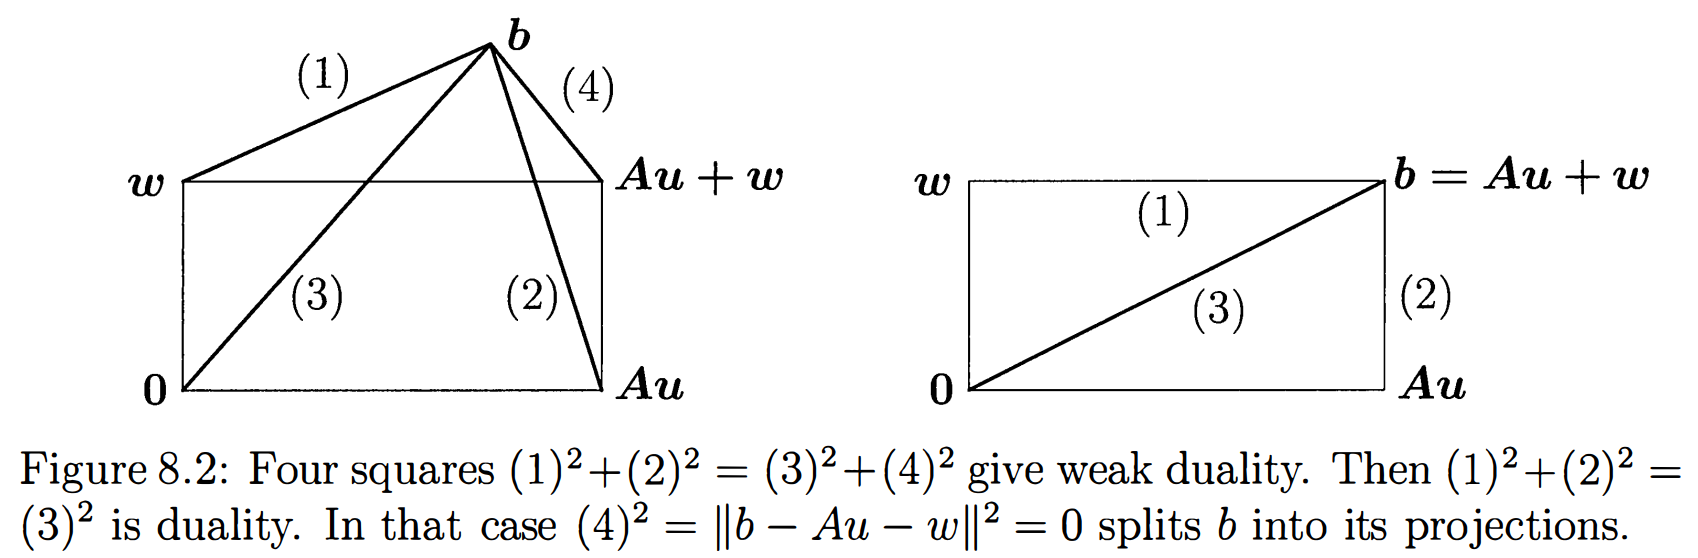
\includegraphics[width=0.9\linewidth]{figs/Strang_wsq_weakduality}
	\caption{Geometric interpretation of weak duality. From Strang.}
	\label{fig:strangwsqweakduality}
\end{figure}

Imagine we have a rectangle, where the perpendicular sides are $Au$ and $w$. The remaining corners of this rectangle are $0$ and $Au + w$. Lines from $b$ to the four corners of this rectangle are vectors $b - X + a$ where $X$ is a corner of the rectangle and $a$ is some offset (since the lines don't all start from 0). 

We can ignore the offset by comparing the vectors' magnitudes. In particular, the diagonal distance starting from either the lower-left or lower-right corner of the rectangle (right side of Fig. \ref{fig:strangwsqweakduality}) is the same, but involve different vectors. The magnitude of each diagonal is the sum of two vectors that meet at $b$. One diagonal connects points $(0, b, Au + w)$, and has magnitude $\parallel b \parallel^2 + \parallel b - (Au + w) \parallel^2$. The other diagonal connects points $(Au, b, w)$, and has magnitude $\parallel b - Au \parallel^2 + \parallel b - w \parallel^2$. Equating these yields the following relationship:

\begin{equation}
\parallel b - Au \parallel^2 + \parallel b-w \parallel^2 = \parallel b \parallel^2 + \parallel b - Au - w \parallel^2 
\end{equation}

At the minimum, we have that $\parallel b \parallel^2 = \parallel b - Au \parallel^2 + \parallel b-w \parallel^2$. This is summarized by the image on the right of Fig. \ref{fig:strangwsqweakduality}, which clearly shows how $Au$ and $w$ are projections of $b$ under this condition:
\begin{align}
\parallel b - Au - w \parallel^2 &= 0 \\
b - Au - w &= 0 \\
Au - w &= b 
\end{align}

The solution $u = \hat{u}$ and $w = e$ gives \textbf{duality}: $\parallel b - A\hat{u} \parallel^2 + \parallel b-e \parallel^2 = \parallel b \parallel^2$. \textbf{Weak duality} is when $\parallel b - A\hat{u} \parallel^2 + \parallel b-e \parallel^2 > \parallel b \parallel^2$. In this scenario, we have a "duality gap" $\parallel b - Au - w \parallel^2$. Duality is achieved when the gap is zero. When this is true, $b = Au - w$, and $b$ becomes a corner of the rectangle, as shown in the right side of Fig. \ref{fig:strangwsqweakduality}. Finally, by Pythagoras' rule: 
\begin{equation}
\parallel b-w \parallel^2 + \parallel b-Au \parallel^2 = \parallel b \parallel^2 = \parallel Au + w \parallel^2,
\end{equation}
which is exactly what happens when we have perfect duality! 

To summarize this section, weighted least squares involves solving two problems:
\begin{enumerate}
	\item Project $b$ onto the column space of $A\hat{u}$:
	\begin{align*}
	\centering
	\min \parallel b-Au \parallel^2
	\end{align*}
	\item Project $b$ across to $e$: \begin{align*}
		\min &\quad \parallel b-w \parallel^2 \\
		\textrm{s.t.} &\quad A^T w = 0
	\end{align*}
\end{enumerate}

The solutions to these problems converge at optimality, as we showed above. At optimality, $\hat{w} = C(b - A\hat{u})$. $C$ is the bridge between the two dual problems and identiies the solutions $\hat{u}$ and $\hat{w}$. Alternatively, we can see the problem as a maximization problem, simply by attaching a negative sign: 
\begin{align}
	\parallel b - e \parallel^2 + \parallel b - A \hat{u} \parallel^2 &= \parallel b \parallel^2 \\
	\parallel b - e \parallel^2 - \parallel b \parallel^2 &= -\parallel b - A \hat{u} \parallel^2 \\
	\therefore \quad \min (\parallel b-e \parallel^2 - \parallel b \parallel^2) \quad &\equiv \quad \max (-\parallel b - A \hat{u} \parallel^2)
\end{align}

\subsection{Minimizing with Constraints using Lagrange's Method}
Imagine we have a line of two springs and one mass and that we wish to minimize the energy in the springs. The constraint is $A^T w = f$, where we have forces $w_1$ and $w_2$, and a mass that exerts external force $f$. The springs are vertically arranged with the mass in between, which causes spring 1 (top) to stretch, and spring 2 (bottom) to compress (Fig. \ref{fig:strangconstrainedsprings}). 

\begin{figure}[H]
	\centering
	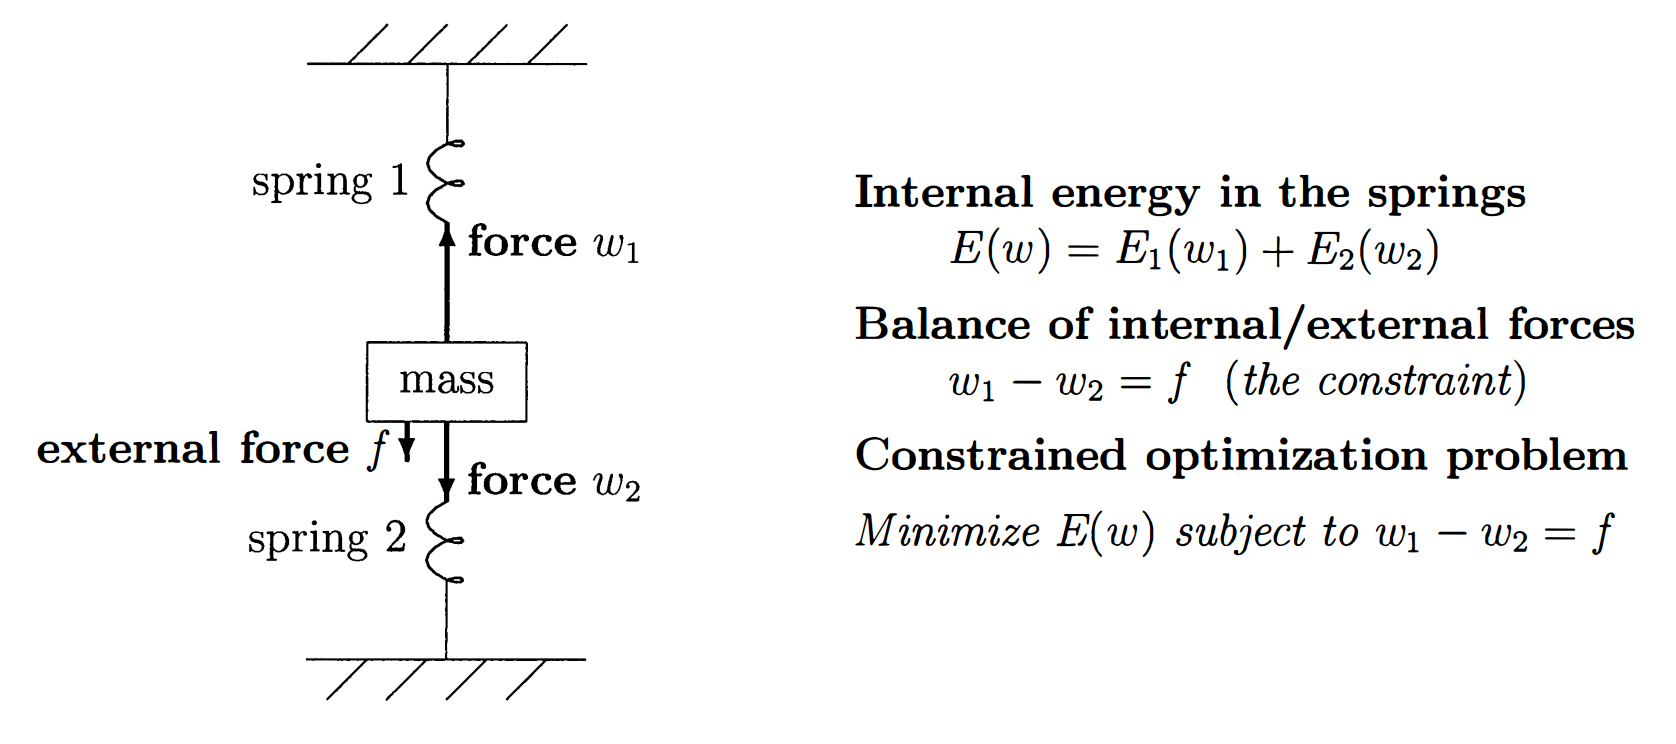
\includegraphics[width=0.8\linewidth]{figs/Strang_constrained_springs}
	\caption{System with two linear springs and one mass.}
	\label{fig:strangconstrainedsprings}
\end{figure}

To solve the force balance equation $w_1 + w_2 = f$, we won't use calculus (setting derivatives to zero), because while we have an energy function $E(w_1 , w_2)$, it is unclear which derivatives we should adjust to achieve force balance. We could make the substitution: $w_2 = w_1 - f$, so that we only minimize over one variable, $w_1$. Here, we will use Lagrange multipliers to \textit{build constraints into the function} by adding an unknown $u$ that enforces our constraint. 

With $n$ constraints on $m$ unknowns, this method has $m + n$ unknowns. We will add a Lagrange multiplier for each constraint. The Lagrange function is:
\begin{equation}
L(w_1, w_2, u) = E_1 (w_1) + E_2 (w_2) - u(w_1 - w_2 - f) = E_1 + E_2 - u (w_1 - w_2 - f)
\end{equation}

Where, $u$ takes a negative sign by convention. $w_2$ takes a negative sign as well, to distinguish the compression of spring 2 from the stretching of spring 1. Note that constraints, the term multiplied by $u$, must equal zero. The Lagrange multiplier $u$ has a special meaning: here, the displacement of the mass. In economics, the selling price for maximal profit. In all problems, $u$ measures the answer's sensitivity (here, the minimum energy $E_{\textrm{min}}$) to changes in constraints. 

Hooke's law tells us that the force in a linear spring is proportional to elongation $e$, so $w = ce$. Work = force $\times$ displacement, and the integral of work is energy. Thus, Work = $ce$, and energy $E$ = $\int$ Work = $\frac{1}{2} ce^2$. Substituting $e = \frac{w}{c}$, we get $E = \frac{w^2}{2c}$. The resulting minimization problem is then:
\begin{align}
\min &\quad E(w) = \frac{w_{1}^2}{2c} + \frac{w_{2}^2}{2c} \\
\textrm{s.t. } &\quad w_1 - w_2 = f \nonumber 
\end{align}

\subsubsection{Geometry of the method}
\begin{figure}[H]
	\centering
	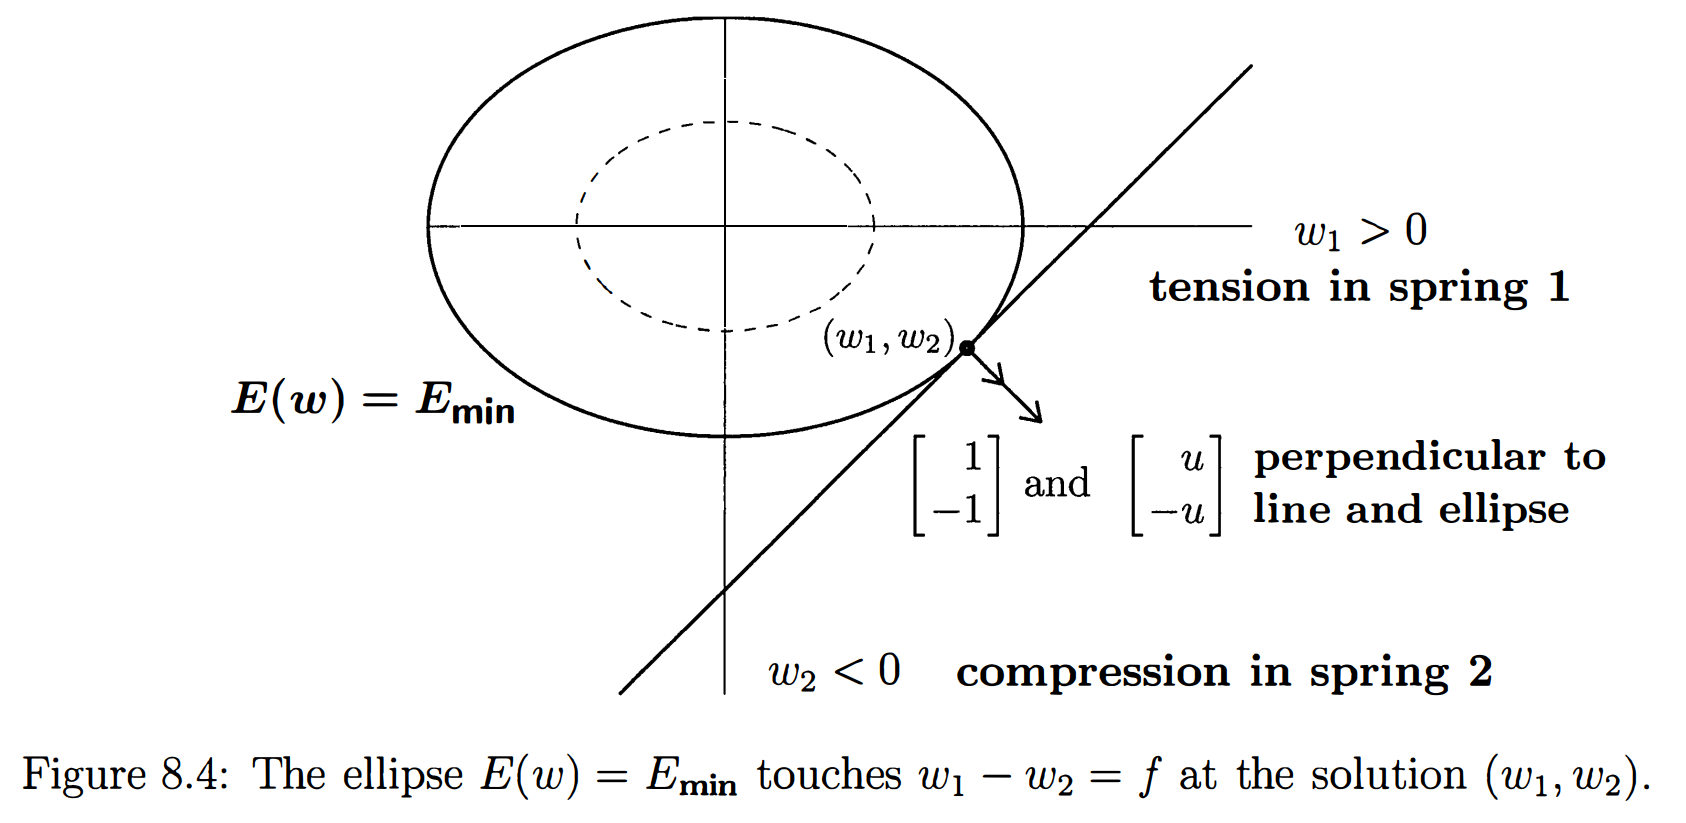
\includegraphics[width=0.9\linewidth]{figs/Strang_constrained_geo}
	\caption{Geometric depiction of $E(w_1, w_2)$ and constraint $w_1 - w_2 = f$.}
	\label{fig:strangconstrainedgeo}
\end{figure}

Notice that $E(w)$ is the equation of an ellipse. We can think of the constraint geometrically in the plane with axes $w_1$ and $w_2$: $E(w)$ is some ellipse in this plane, and $w_1 - w_2 = f$ is a line with positive slope and negative y-intercept (Fig. \ref{fig:strangconstrainedgeo}). The solution is achieved when the line meets the ellipse at a right-angle. At this point $(w_1 , w_2)$, there are two vectors of interest that describe the rate of change of the ellipse and line with respect to $w_1$ and $w_2$. One is perpendicular to the line: \begin{equation*}
\begin{bmatrix}
\partial l / \partial w_1 \\ \partial l / \partial w_1 
\end{bmatrix} = \begin{bmatrix}
1 \\ -1 
\end{bmatrix}, \quad l = w_1 - w_2 - f = 0
\end{equation*}

The second is perpendicular to the ellipse, and arises from the gradient of $E(w)$:
\begin{align*}
L(w_1, w_2, u) &= E_1 + E_2 - u (w_1 - w_2 - f) \\ 
\frac{\partial L}{\partial w_1} &= \frac{\partial E}{\partial w_1} - u = 0 \\
\frac{\partial L}{\partial w_2} &= \frac{\partial E}{\partial w_2} + u = 0 \\
\begin{bmatrix}
\partial E / \partial w_1 \\ \partial E / \partial w_2 
\end{bmatrix} &= \begin{bmatrix}
u \\ -u
\end{bmatrix}
\end{align*}

The above gives us $w_1$ and $w_2$ as follows:
\begin{align}
\frac{\partial E}{\partial w_1} &= \frac{\partial}{\partial w_1} \frac{w^{2}_{1}}{2c_{1}} = \frac{w_{1}}{c_{1}} \\
\therefore \begin{bmatrix}
\partial E / \partial w_1 \\ \partial E / \partial w_2 
\end{bmatrix} &= \begin{bmatrix}
w_1 / c_1 \\ w_2 / c_2 
\end{bmatrix} = \begin{bmatrix}
u \\ -u
\end{bmatrix} \\ 
w_1 = c_1 u, &\quad w_2 = -c_2 u \\
w_1 - w_2 &= f = c_1 u + c_2 u = (c_1 + c_2)u 
\end{align}

$c_1 + c_2$ is the stiffness matrix $A^T C A$, which we discussed in Section \ref{Weighted Least Squares}. Since the problem is small, $K = A^T C A$ is just $1 \times 1$: 
\begin{equation*}
A^T = \begin{bmatrix}
1 \\ -1
\end{bmatrix}, \quad K = A^T C A = \begin{bmatrix}
1 \\ -1
\end{bmatrix}\begin{bmatrix}
c_1 & \\ & c_2 
\end{bmatrix} \begin{bmatrix}
1 \\ -1 
\end{bmatrix} = \begin{bmatrix}
c_1 + c_2
\end{bmatrix}
\end{equation*}

We now find the forces $w_1$ and $w_2$:
\begin{align*}
Ku &= f \quad \implies \quad u = \frac{f}{c_{1} + c_{2}} \\
w_1 &= c_1 u = \frac{c_1 f}{c_1 + c_2}, \quad w_2 = -c_2 u = -\frac{c_2 f}{c_1 + c_2} \\ 
E_{\textrm{min}} &= \frac{w_{1}^2}{2c} + \frac{w_{2}^2}{2c} = \frac{c_1 f^2}{2 (c_1 + c_2)^2} + \frac{c_2 f^2}{2 (c_1 + c_2)^2} \\
 &= \frac{f^2}{2 (c_1 + c_2)}
\end{align*}

Above, we mentioned that $u$ measures the sensitivity of $E_{\textrm{min}}$ to changes in the constraint, $f$. We can show this by computing the derivative $\frac{dE_{\textrm{min}}}{df}$:
\begin{align}
\frac{dE_{\textrm{min}}}{df} &= \frac{d}{df} \left(\frac{f^2}{2 (c_1 + c_2)}\right) \nonumber \\
&= \frac{f}{c_1 + c_2} = u
\end{align}

\subsection{The Fundamental Problem}
This is what Strang describes as the \textit{fundamental problem of scientific computing}: the full linear case with $m$ springs. Each spring experiences a force $w_i$, which we can represent as $w = (w_1, \dotsm, w_m)$. We have $n$ constraints for force balance, $A^{T}w = (f_1, \dotsm, f_n)$, enforced by $n$ Lagrange multipliers $u = (u_1, \dotsm, u_n)$.

Let $C$ be a matrix with masses $c_1, \dotsm, c_m$ on the diagonal and zeroes everywhere else. Then, the total energy function for $m$ springs is given by: $E(w) = \frac{1}{2}w^T C^{-1} w$. Our Lagrange function is thus:
\begin{equation}
L(w, u) = \frac{1}{2}w^T C^{-1} w - u^{T}(A^{T}w - f)
\end{equation}

The minimizer $w$ is found by setting the $m+n$ partial derivatives of $L$ to zero:
\begin{align}
\frac{\partial L}{\partial w} &= C^{-1}w - Au = 0 \label{fundamental_pLpw}\\
\frac{\partial L}{\partial u} &= -A^{T}w + f = 0 \label{fundamental_pLpu}
\end{align}

From Eq. \ref{fundamental_pLpw}, we have that $w = Ce = CAu$, which implies that $e = Au$. Eq. \ref{fundamental_pLpu} indicates that $f = A^{T}w$. Together, we have that:
\begin{equation}
A^T C A u = A^T C e = A^T w = f
\end{equation}

Least squares problems have $e = b - Au$, which appears in $E$ as:
\begin{equation*}
E(b, w) = \frac{1}{2}w^T C^{-1} w - b^T w
\end{equation*}

The derivatives of $L$ (with $u$ positive) are:
\begin{align}
\frac{\partial L}{\partial w} &= C^{-1}w + Au - b = 0 \\
\frac{\partial L}{\partial u} &= -A^{T}w - f = 0 \\
\begin{bmatrix}
C^{-1} & A \\ A^{T} & 0 
\end{bmatrix} &\begin{bmatrix}
w \\ u
\end{bmatrix} = \begin{bmatrix}
b \\ f
\end{bmatrix}
\end{align}

The vector $(w, u)^{T}$ has size $m + n$, since $w$ has $m$ components and $u$ has $n$. If $C$ is positive definite, and $A$ has full column rank (all columns are independent, Rank($A$) = $n$), then $A^{T}CA$ and $S$ are invertible. We can factor $S$ into three parts as follows:
\begin{equation*}
S = \begin{bmatrix}
C^{-1} & A \\ A^{T} & 0 
\end{bmatrix} = \begin{bmatrix}
I & 0 \\ A^{T}C & I
\end{bmatrix} \begin{bmatrix}
C^{-1} & 0 \\ 0 & -A^{T}CA
\end{bmatrix}\begin{bmatrix}
I & CA \\ 0 & I
\end{bmatrix}
\end{equation*}

$S$ is invertible when both block columns have full rank. Otherwise, it can be singular. 

\section{Regularized Least Squares}

Regularized least squares is a special case of weighted least squares:
\begin{align*}
\textrm{\textbf{Ordinary LSQ}} \quad & \min \parallel Au - b \parallel^2 \\
\textrm{Solve: } & A^TA\hat{u} = A^T b \\
\textrm{\textbf{Weighted LSQ}} \quad & \min (b-Au)^{T} C (b-Au) \\
\textrm{Solve: } & A^T C A\hat{u} = A^T C b \\
\textrm{\textbf{Regularized LSQ}} \quad & \min \parallel Au - b \parallel^2 + \alpha \parallel Bu-d \parallel^2 \\
\textrm{Solve: } & (A^T A + \alpha B^{T}B)\hat{u} = A^{T}b + \alpha B^{T}d
\end{align*}

We can rewrite the regularized LSQ equations to resemble those for weighted LSQ by replacing $A$ in the latter by $[A \ B]^T$:
\begin{equation}
\begin{bmatrix}
A^T & B^T
\end{bmatrix} \begin{bmatrix}
I & 0 \\ 0 & \alpha I 
\end{bmatrix} \hat{u} = \begin{bmatrix}
A^T & B^T
\end{bmatrix}  \begin{bmatrix}
I & 0 \\ 0 & \alpha I 
\end{bmatrix} \begin{bmatrix}
b \\ d
\end{bmatrix}
\end{equation}

Where, the weighting matrix $C =  \begin{bmatrix}
I & 0 \\ 0 & \alpha I 
\end{bmatrix}$. There are two important applications that lead to this sum of two squares $(A^T A, B^{T}B)$:
\begin{enumerate}
	\item If $A^{T}A$ is ill-conditioned, e.g. very large ratio of largest to smallest eigenvalues, $m < n$, $A^{T}A$ is singular. \\
	Regularization acts to 'reduce the noise.' Normally, as $\alpha$ is increased, $\parallel \hat{u} \parallel$ decreases and $\parallel A\hat{u} - b \parallel$ increases. The \textbf{Discrepancy Principle} selects $\alpha$ so that $\parallel \hat{u} \parallel$ decreases and $\parallel A\hat{u} - b \parallel \approx $ expected noise (uncertainty in $b$).
	\item As $\alpha \rightarrow \infty$, $Bu \rightarrow d$. The limiting $\hat{u}_{\infty}$ solves 
	\begin{align}
	\min &\quad \parallel Au-b \parallel^2 \\
	\textrm{s.t.} &\quad Bu=d \nonumber 
	\end{align}
\end{enumerate}

\subsection{Example: Large Penalty Enforced $Bu=d$}
\begin{align*}
\textrm{Problem:} \quad \min &\quad \parallel Au \parallel^2 = u_{1}^{2}+u_{2}^{2} \\
\textrm{s.t.} &\quad Bu = u_1 - u_2 = 8
\end{align*}
Let $A = \begin{bmatrix}
1 & 0 \\ 0 & 1
\end{bmatrix}, \quad b = \begin{bmatrix}
0 \\ 0
\end{bmatrix}, \quad B = \begin{bmatrix}
1 & -1
\end{bmatrix}, \quad d = \begin{bmatrix}
8
\end{bmatrix}$.

\begin{align*}
A^T A = I, \quad B^T B = \begin{bmatrix}
1 & -1 \\ -1 & 1
\end{bmatrix}, \quad &\begin{bmatrix}
1+\alpha & -\alpha \\ -\alpha & 1+\alpha
\end{bmatrix}\begin{bmatrix}
u_1 \\ u_2 
\end{bmatrix} = \begin{bmatrix}
8\alpha \\ -8\alpha
\end{bmatrix} = \alpha B^T d \\
u_1 + u_2 = 0, \quad &(1 + 2\alpha)u_1 = 8\alpha \\
&u_1 = \frac{8\alpha}{1+2\alpha} = \frac{4}{1 + \frac{\alpha}{2}} = 4 - \frac{4}{2\alpha} + \dotsm \rightarrow u_1 = 4
\end{align*}

The order is of order $1/\alpha$, so we need large $\alpha$.

\subsection{The Pseudoinverse}
Suppose $A$ is $m \times n$ and $b$ has $m$ components. The normal equations $A^{T}A\hat{u} = A^{T}b$ only give $\hat{u}$ when $A^{T}A$ is invertible. Otherwise, we can use the pseudoinverse to find the best solution $u^{+}$. This works even when $A$ is not full rank and $A^{T}A$ is singular

\subsubsection{What is $u^{+}$?}
$u^{+} = A^{+}b$ provides the \textbf{shortest} vector that solves $A^{T}Au^{+} = A^{T}b$. 

Other solutions, longer than $u^{+}$, have components in the nullspace of $A$. $u^{+}$ is \textbf{the particular solution with no nullspace component}. The \textbf{pseudoinverse} of $A$ is a matrix $A^{+}$, which produces $u^{+} = A^{+}b$. If $A$ is square and invertible, then $u^{+} = u = A^{-1}b$, and $A^{+} = A^{-1}$. 

If $A$ has independent columns, but $m < n$, then $\hat{u} = (A^{T}A)^{-1}A^{T}b$ is the only solution, where $A^{+} = (A^{T}A)^{-1}A^{T}$. If $A$ has dependent columns and thus a nonzero nullspace: any $Au$ is a linear combination of the columns of $A$, but if the columns are dependent, then there exists a nonzero vector $x$ such that $Ax = 0$, and so $x \in \textrm{Nul}(A)$ and Nul($A$) $\neq \{0\}$.

\begin{figure}[H]
	\centering
	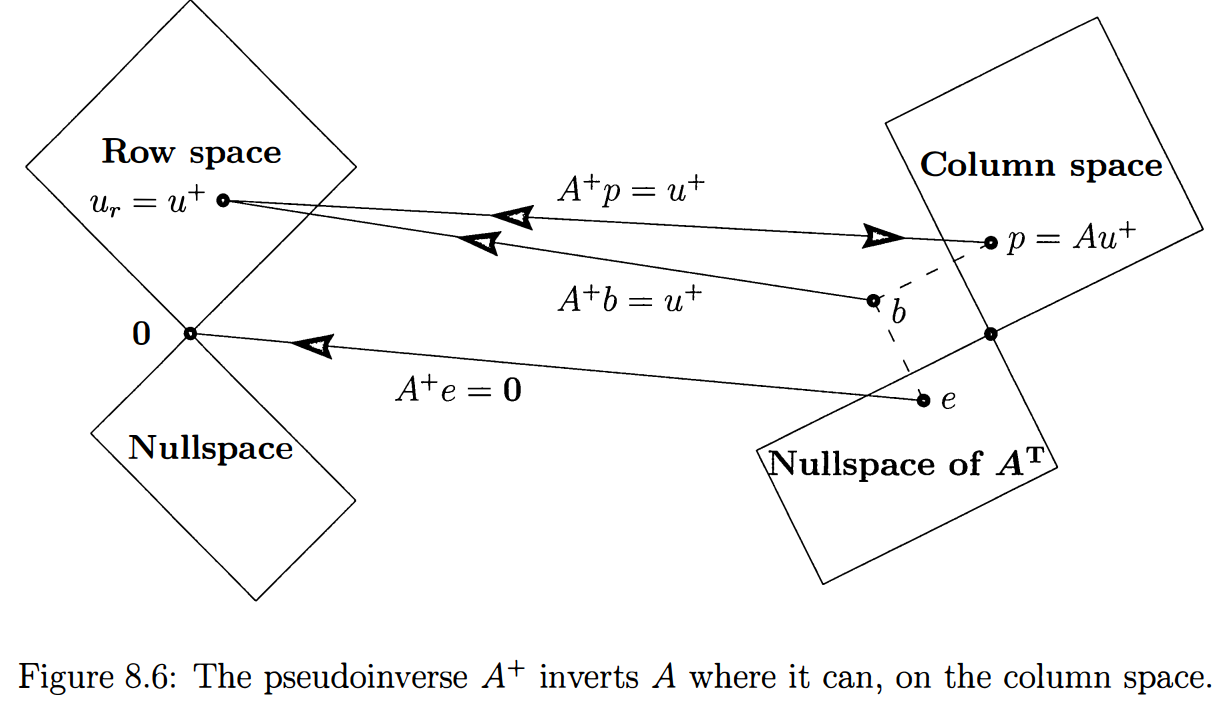
\includegraphics[width=0.8\linewidth]{figs/Strang_pseudoinverse}
	\caption{$Au$ takes vectors $u = u_{\textrm{row}} + u_{\textrm{null}}$ to the column space of $A$. Since $u_{\textrm{row}}$ and $u_{\textrm{null}}$ are orthogonal, a non-zero $u_{\textrm{null}}$ increases $\norm{u}^{2}$. Thus, $u^{+} = u_{\textrm{row}}$}. 
	\label{fig:strangpseudoinverse}
\end{figure}

$u^{+}$ solves $Au^{+} = p$, where $p$ is the projection of $b$ onto the column space of $A$. The error $\norm{e} = \norm{b-p} = \norm{b-Au^{+}}$ is minimized by $u^{+}$. In summary, $u^{+}$ is in the row space (to be as short as possible), and $Au^{+} = p$ (to be as close to $b$ as possible); $u^{+}$ minimizes $e$ and solves $A^T A u^{+} = A^T b$. 

\subsubsection{Singular Value Decomposition (SVD)}
One method to compute $u^{+}$ is by SVD. Let's review diagonalization and SVD. 

Recall the \textbf{Diagonalization Theorem}:
\begin{itemize}
	\item An $n \times n$ matrix $A$ is diagonalization if and only if $A$ has $n$ linearly independent eigenvectors.
	\item $A = PDP^{-1}$ with $D$ being a diagonal matrix, if and only if the columns of $P$ are $n$ linearly independent eigenvectors of $A$. Then, the entries of $D$ are the corresponding eigenvalues of $A$ for the eigenvectors in $P$. 
\end{itemize}

\paragraph{Diagonalization of Symmetric Matrices \\}
Furthermore, if $A$ is symmetric, then:
\begin{itemize}
	\item $A^{T} = A$
	\item All eigenvectors from different eigenspaces (i.e. corresponding to different eigenvalues) are \textbf{orthogonal} to each other.
	\item $A = PDP^{-1}$, but $P$ is square and has orthonormal columns $\implies$ $P$ is an \textit{orthogonal matrix}, and $P^{-1} = P^{T}$.
	\item $A$ is orthogonally diagonalizable if and only if $A$ is symmetric. 
\end{itemize}

We can prove that, for symmetric $A$, two given eigenvectors $v_1$ and $v_2$ are orthogonal:
\begin{align*}
\lambda_1 v_1 \cdot v_2 &= (\lambda_1 v_1)^{T} v_2 = (Av_1)^{T}v_2 \quad \leftarrow \lambda_1 v_1 = A v_1 \\
&= (v_{1}^{T}A^{T})v_2 = v_{1}^{T}(Av_2) = v^{T}_{1}(Av_{2}) \quad \leftarrow A^T = A \\
&= v_{1}^{T} \lambda_{2}v_{2} = \lambda_{2}v_{1}^{T}v_{2} = \lambda_{2}v_{1} \cdot v_{2} \\
(\lambda_{1} - \lambda_{2})v_{1}\cdot v_{2} &= 0 \\
\lambda_{1} - \lambda_{2} &\neq 0 \quad \implies \quad v_{1} \cdot v_{2} = 0
\end{align*}

An $n \times n$ matrix $A$ is \textit{orthogonally diagonalizable} if there are an orthogonal matrix $P$ with $P^{-1} = P^{T}$, and a diagonal matrix $D$ such that
\begin{equation}
A = PDP^{T} = PDP^{-1}
\end{equation}

This requires $n$ linearly independent and orthonormal eigenvectors. This is possible when $A$ is symmetric:
\begin{equation*}
A^{T} = (PDP^{T})^{T} = P^{TT}D^{T}P^{T} = PDP^{T} = A
\end{equation*}

\paragraph{Spectral decomposition of a Symmetric Matrix \\}
\textbf{Spectral decomposition} is possible when $A$ is symmetric:
\begin{align*}
A = PDP^{T} &= \begin{bmatrix}
u_1 \dotsm u_n
\end{bmatrix} \textrm{diag}(\lambda_1 , \dotsm, \lambda_n) \begin{bmatrix}
u_{1}^{T} \\ \vdots \\ u_{n}^{T}
\end{bmatrix} \\
&= \begin{bmatrix}
\lambda_{1}u_{1} \dotsm \lambda_{n}u_{n} 
\end{bmatrix}\begin{bmatrix}
u_{1}^{T} \\ \vdots \\ u_{n}^{T}
\end{bmatrix} \\
&= \lambda u_{1} u_{1}^{T} + \dotsm + \lambda_{n}u_{n}u_{n}^{T}
\end{align*}

Here, each matrix $u_{i}u_{i}^{T}$ is $1 \times 1$ and is a \textbf{projection matrix} in the sense that, $u_{i}u_{i}^{T}x$, for all $x \in \mathds{R}^{n}$, is the orthogonal projection of $x$ onto the subspace spanned by $u_{i}$.

\paragraph{SVD of an $m \times n$ matrix $A$ \\}

Let's finally talk about SVD. The key insight is that, even if we can't factorize an $m \times n$ matrix $A$ as $A = PDP^{-1}$, \textbf{we can always perform SVD to get $\mathbf{A = QDP^{-1}}$. }

Let $A$ be an $m \times n$ matrix. Then, $A^{T}A$ is symmetric, and can be orthogonally diagonalized as $A^{T}A = PDP^{T}$. Let $\{v_1, \dotsm v_{n} \}$ be an orthonormal basis for $\mathds{R}^{n}$ consisting of eigenvectors of $A^{T}A$. Let $\lambda_{1}, \dotsm, \lambda_{n}$ be the corresponding eigenvalues. Then,
\begin{align*}
\norm{Av_i}^{2} &= (Av_i)^{T}(Av_i) = v_{i}^{T}A^{T}Av_{i} \\
&= v_{i}^{T} (\lambda_{i}v_{i}) \quad \leftarrow Av_{i} = \lambda_{i}v_{i} \\
&= \lambda_{i} v_{i}^{T}v_{i} = \lambda_{i} \quad \leftarrow v_{i}^{T}v_{i} = 1 \\
\implies \quad \lambda_{i} \geq 0
\end{align*}

The \textbf{singular values} of $A$ are the square roots of the eigenvalues of $A^{T}A$: $\sigma_{i} = \sqrt{\lambda_{i}} = \sqrt{\norm{Av_i}^{2}} = \norm{Av_i}$. Therefore, we can also see that $\sigma_{i}$ is the length of the vector $Av_{i}$. 

Since $v_i$ and $\lambda_{j}v_j$ are orthogonal while $i \neq j$,
\begin{equation*}
(Av_i)^{T}(Av_j) = v_{i}^{T}A^{T}Av_{j} = v_{i}^{T}(\lambda_j v_{j}) = 0
\end{equation*}

This shows that $\{Av_{1}, \dotsm, Av_{n} \}$ is an \textbf{orthogonal set}. The lengths of $Av_{i}$ is given by the corresponding singular values of $A$. Typically, we arrange the singular values in order of decreasing magnitude, so that:
\begin{align*}
&\lambda_{1} \geq \lambda_{2} \geq \dotsm \lambda_{n} \geq 0 \\
&\sigma_{1} \geq \sigma_{2} \geq \dotsm \sigma_{n} \geq 0 
\end{align*}

If $A$ has $r$ non-zero singular values, then Rank($A$) = $r$, and $\{Av_{1}, Av_{2}, \dotsm, Av_{r} \}$ is an \textbf{orthogonal basis} for Col($A$). To show that the basis is $r-$dimensional, rather than $n-$dimensional, we will show that a vector $y$ in Col($A$) can be expressed as a linear combination of $\{Av_{1}, \dotsm, Av_{r} \}$:
\begin{align*}
x &= c^{T}v = c_{1}v_{1} + \dotsm + c_{n}v_{n} \\
y &= Ax = c_{1}Av_{1} + \dotsm c_{r}Av_{r} + c_{r+1}Av_{r+1} + \dotsm + c_{n}Av_{n} \\
&= c_{1}Av_{1} + \dotsm + c_{r}Av_{r} + 0 + \dotsm + 0
\end{align*}

Thus, $y$ is in Span$\{Av_{1}, \dotsm, Av_{r} \}$. Hence, Rank($A$) = dim(Col($A$)) = $r$.

\paragraph{SVD \\}
Let $A$ be an $m \times n$ matrix of rank $r$. Then, there is an $m \times n$ matrix $\Sigma$,
\begin{equation*}
\Sigma = \begin{bmatrix}
D & 0 \\ 0 & 0
\end{bmatrix}
\end{equation*}
for which the diagonal entries in $D$ are the first $r$ (i.e. the non-zero) singular values of $A$, where
\begin{equation*}
\sigma_{1} \geq \sigma_{2} \geq \dotsm \geq \sigma_{r} > 0
\end{equation*}
Finally, there is an $m \times m$ orthogonal matrix $U$ and an $n \times n$ matrix $V$ such that:
\begin{equation}
A = U \Sigma V^{T}
\end{equation}

$U$ and $V$ are not uniquely determined by $A$, and are referred to as the left- and right-singular vectors of $A$, respectively. We prove SVD below, starting with the assumption that $A$ is a $m \times n$ matrix with eigenvalues $\lambda_{i}$, corresponding eigenvectors $v_{i}$, and $r$ non-zero singular values $\sigma_{i}$. As shown above, $\{Av_{1}, \dotsm, Av_{r} \}$ will be an orthogonal basis for Col($A$). 

Normalize each $Av_{i}$ to obtain an orthonormal basis $U$:
\begin{align*}
U &= \{u_{1}, \dotsm, u_{r} \}, \textrm{ where} \\
 u_{i} &= \frac{Av_{i}}{\norm{Av_{i}}} = \frac{Av_{i}}{\sigma_{i}} \\
 Av_{i} &= \sigma_{i}u_{i}, \quad 1 \leq i \leq r 
\end{align*}

Extend $U$ to a basis of $\mathds{R}^{m}$: 
\begin{equation*}
U = \begin{bmatrix}
u_{1} & u_{2} & \dotsm & u_{m} 
\end{bmatrix} 
\end{equation*}
Let $V = \begin{bmatrix}
	v_{1} & v_{2} & \dotsm & v_{n}
\end{bmatrix}$. Then, $U$ and $V$ are both orthogonal matrices. We also have that
\begin{align*}
AV &= \begin{bmatrix}
Av_{1} & \dotsm & Av_{r} & 0 & \dotsm & 0
\end{bmatrix} = \begin{bmatrix}
\sigma_{1}u_{1} & \dotsm & \sigma_{r}u_{r} & 0 & \dotsm & 0
\end{bmatrix}
\end{align*}

Let $D$ be a diagonal matrix with diagonal entries $\sigma_{1}, \dotsm, \sigma_{r}$. Then,
\begin{align*}
U\Sigma &= \begin{bmatrix}
u_{1} & u_{2} & \dotsm & u_{m}
\end{bmatrix} \begin{bmatrix}
D & \textrm{$n - r$ columns of $0$} \\
\textrm{$m-r$ rows of $0$} & 0 \\
\end{bmatrix} \\
&= \begin{bmatrix}
\sigma_{1}u_{1} & \sigma_{2}u_{2} & \dotsm & \sigma_{r}u_{r} & 0 & \dotsm & 0
\end{bmatrix} \\
&= AV \\
V^{-1} = V^{T} \quad \implies &\quad U\Sigma V^{T} = AVV^{T} = A 
\end{align*}

\subsubsection{Computing $u^{+}$ with SVD}

\begin{equation}
\textrm{\textbf{SVD:}} \quad A = U\Sigma V^T = \begin{bmatrix}
U_{\textrm{col}} & U_{\textrm{null}}
\end{bmatrix} \begin{bmatrix}
\Sigma_{\textrm{pos}} & 0 \\ 0 & 0
\end{bmatrix} \begin{bmatrix}
V_{\textrm{row}} & V_{\textrm{null}}
\end{bmatrix}^{T}
\end{equation}

$U$ and $V$ are square matrices that have orthonormal columns: $U^{T}U = I$ and $V^{T}V = I$. $U_{\textrm{col}}$ and $V_{\textrm{row}}$ are bases for the column and row spaces of $A$, respectively, and have dimensions $r = \textrm{Rank}(A)$. The other 'null' columns are in the nullspaces of $A^T$ ($U_{\textrm{null}}$) and $A$ ($V_{\textrm{null}}$). 

The pseudoinverse of $A$ is computed as:
\begin{equation}
A^{+} = V_{row}(\Sigma_{pos})^{-1}U_{col}^{T}
\end{equation}

Where, $\Sigma_{pos}$ is a diagonal matrix containing the \textit{positive} singular values of $A$. $A^{+}b = u^{+}$ puts $u^{+}$ in the row space of $A^{+}$. 

\subsubsection{Computing $u^{+}$ with Tychonov Regularization}
SVD may not always be the most practical approach for solving the normal equations. When $A^{T}A$ is singular (the problem here), we can add a small multiple of $\alpha I$, producing what is known as \textbf{Tychonov Regularization}:
\begin{align}
\min &\quad \norm{Au-b}^{2} + \alpha \norm{u}^{2} \\
\textrm{s.t.} &\quad (A^{T}A + \alpha I)\hat{u}_{\alpha} = A^{T}b \nonumber 
\end{align}

This is similar to our original formulation of regularized LSQ, with $B = I$, $d=0$, and $\alpha \norm{u}^{2}$ as the regularizing term. When $\alpha$ is small, we prioritize the minimization of $\norm{Au-b}^{2}$. In the limit that $\alpha \rightarrow 0$, we have that 
\begin{align*}
\lim\limits_{\alpha \rightarrow 0} \hat{u}_{\alpha} &= \lim\limits_{\alpha \rightarrow 0} (A^{T}A + \alpha I)^{-1} A^{T}b \\
&= (A^{T}A)^{-1}A^{T}b = A^{+}b \\
&= u^{+} 
\end{align*}

We don't get $u^{+}$ exactly, with small $\alpha > 0$. There is also uncertainty in $b$. The presence of a small $\alpha$ in $(A^{T}A + \alpha I)^{-1}A^{T}$ introduces small, non-zero singular values along the diagonal of our singular values matrix $\Sigma$ in SVD. Importantly, $\frac{\sigma}{\sigma^{2} + \alpha} \rightarrow \frac{1}{\sigma}$ while $\alpha > 0$, but stays zero if $\sigma = 0$. 

\subsection{Tychonov Regularization}
This section discusses how to choose $\alpha$. The key ideas are as follows:
\begin{enumerate}
	\item There is noise in measurement of $b$, represented by an error $e$. 
	\item $e$ is amplified when $A$ is ill-conditioned (e.g. singular $A^{T}A$) and $\alpha = 0$ (no regularization). This is why we use regularization. 
	\item Choosing an appropriate $\alpha$, we can stabilize the problem by adding $\alpha I$. However, if $\alpha$ is too small, then $e$ will still grow with $A^{-1}$. If $\alpha$ is too large, we lose accuracy on $\hat{u}$. 
\end{enumerate}

We will refer to multiple versions of the solution using the notation $\hat{u}_{i}^{j}$, where $i$ represents our choice of $\alpha$, and $j$ the expected size of uncertainty in $b$. For instance, $\hat{u}_{0}^{0}$ refers to the solution without regularization or measurement error. On the other hand, $\hat{u}_{\alpha}^{e}$ is the solution attained from data with measurement error $e$, using regularization parameter $\alpha$. 

\subsubsection{Error bounds in $\hat{u}$}
\paragraph{Error bounds when $A$ is a scalar. \\ }
Let's first see how different we expect the solution $\hat{u}$ to be in the two extreme cases: $\hat{u}_{0}^{0}$ (no error, no regularization) and $\hat{u}_{\alpha}^{e}$ (error and regularization).
\begin{align}
\hat{u}_{0}^{0} - \hat{u}_{\alpha}^{e} &= \hat{u}_{0}^{0} - \hat{u}_{0}^{0} + \hat{u}_{0}^{0} - \hat{u}_{\alpha}^{e} \\
\norm{\hat{u}_{0}^{0} - \hat{u}_{0}^{\alpha}} \leq C\alpha\norm{b} &\qquad \norm{\hat{u}_{\alpha}^{0} - \hat{u}_{\alpha}^{e}} \leq \frac{\norm{e}}{2\sqrt{\alpha}} \label{errorbounds}
\end{align}

Where, $C$ is a constant that we will define below. Let's first prove the error bounds in Eq. \ref{errorbounds} when $A$ is a scalar $s$. Then, $A^{T}A = s^{2}$. When noise is absent from measurements:
\begin{align}
\textrm{Without regularization:} &\quad s^2 \hat{u}_{0}^{0} = sb \\
\textrm{With regularization:} &\quad (s^{2}+\alpha)\hat{u}_{\alpha}^{0} = sb \\
\hat{u}_{0}^{0} - \hat{u}_{\alpha}^{0} &= \frac{b}{s} - \frac{sb}{s^{2}+\alpha} \nonumber \\
&= \frac{b(s^{2}+\alpha)-s^{2}b}{s(s^{2}+\alpha)} \nonumber \\
&= \frac{\alpha b}{s(s^{2}+\alpha)} \leq C \alpha b, \quad C = \frac{1}{s^{3} + s\alpha} \label{errorbounds_scalar_nonoise}
\end{align}

Eq. \ref{errorbounds_scalar_nonoise} shows that, in the absence of measurement noise, the error associated with regularization is proportional to $\alpha$, i.e. $O(\alpha)$. $C$ scales steeply with $1/s^{3}$. We perform the same procedure to compare the effect of measurement noise:

\begin{align}
\textrm{Without noise:} &\quad (s^{2} + \alpha)\hat{u}_{\alpha}^{0} = sb \\
\textrm{With noise:} &\quad (s^{2} + \alpha)\hat{u}_{\alpha}^{e} = s(b-e) \\ 
\hat{u}_{\alpha}^{0} - \hat{u}_{\alpha}^{e} &= \frac{sb}{s^{2}+\alpha} - \frac{s(b-e)}{s^{2} + \alpha} \nonumber \\ 
&= \frac{s}{s^{2}+\alpha}e 
\end{align}
{The maximum value of $s/(s^{2}+\alpha)$ will determine the bound. We can find this value by setting its derivative to zero.
\begin{align}
0 &= \frac{d}{ds}\frac{s}{s^{2}+\alpha} = (s^{2}+\alpha)^{-1} - s(s^{2}+\alpha)^{-2}(2s) \nonumber \\
&= \frac{1}{s^{2}+\alpha} - \frac{2s^{2}}{(s^{2}+\alpha)^{2}} \nonumber \\
\frac{2s^{2}}{(s^{2}+\alpha)^{2}} &= \frac{1}{s^{2}+\alpha} \implies 2s^{2} = s^{2} + \alpha, \quad \therefore s = \sqrt{\alpha} \nonumber \\
\therefore \frac{s}{s^{2}+\alpha} &\leq  \frac{1}{2\sqrt{\alpha}} \label{errorbound_scalar_withnoise} 
\end{align}

\paragraph{Error bounds when $A$ is a matrix. \\}
SVD of $A$ produces orthonormal bases $\{u_{1}, u_{2}, \dotsm \}$ and $\{v_{1}, v_{2}, \dotsm \}$, with $Av_{j} = \sigma_{j}u_{j}$ and $A^{T}u_{j} = \sigma_{j}v_{j}$. Note that, unlike before, we are not using $v_i$ to refer to the eigenvectors of $A$; instead, they are the right-singular vectors of $A$. 

We can apply SVD to rewrite the regularized LSQ problem in terms of $u_{j}$ and $v_{j}$:
\begin{align}
(A^{T}A + \alpha I)\hat{u}^{0}_{\alpha} &= A^{T}b \nonumber \\
b = B_{1}u_{1} + B_{2}u_{2} + \dotsm, &\quad \hat{u}^{0}_{\alpha} = U_{1}v_{1} + U_{2}v_{2} + \dotsm \nonumber \\ 
(A^{T}A + \alpha I)U_{j}v_{j} &= A^{T}B_{j}u_{j}  \\
U_{j} A^{T}A v_{j} + U_{j} \alpha I v_{j} &= \sigma_{j}B_{j}v_{j} \nonumber \\
U_{j} \sigma_{j} A^{T} u_{j} + U_{j} \alpha v_{j} &=  \nonumber \\
U_{j} \sigma_{j} (\sigma_{j}v_{j}) + U_{j} \alpha v_{j} &= \nonumber \\
U_{j}v_{j}(\sigma_{j}^{2}+\alpha) &= \nonumber \\
U_{j}(\sigma_{j}^{2}+\alpha) &= \sigma_{j}B_{j} \\
\implies U_{j} &= \frac{\sigma_{j}}{\sigma_{j}(\sigma_{j}^{2}+\alpha)}B_{j} = \frac{\sigma_{j}}{\sigma_{j}^{3}+\sigma_{j}\alpha}B_{j} \label{errorbound_matrix_nonoise}
\end{align}

Eq. \ref{errorbound_matrix_nonoise} is identical to what we saw for the scalar case (Eq. \ref{errorbounds_scalar_nonoise}) if $s = \sigma_{j}$. Likewise, the results in the presence of noise are also similar to the scalar case. To get the total difference between either solution group, we need to sum each of the $U_{j}$ coefficients:
\begin{align}
\hat{u}_{0}^{0} - \hat{u}_{\alpha}^{0} &= \sum_{j=1}^{\infty} \frac{\alpha B_{j}}{\sigma_{j}(\sigma_{j}^{2}+\alpha)} v_{j} \\
\hat{u}_{\alpha}^{0} - \hat{u}_{\alpha}^{e} &= \sum_{j=1}^{\infty} \frac{s_{j} E_{j}}{s_{j}^{2} + \alpha} v_{j}
\end{align}

Where, in the presence of noise, we replace $b$ with $e = E_{1}v_{1} + E_{2}v_{2} \dotsm$. The norm of either sum is a sum of squares wherein the $v_{j}$ terms disappear because they are orthonormal: $\sum_{j=1}^{\infty} v_{j}^{2} = 1$. Hence,

\begin{align}
\norm{\hat{u}_{0}^{0} - \hat{u}_{\alpha}^{0}}^{2} &= \sum_{j=1}^{\infty} \left(\frac{\alpha B_{j}}{\sigma_{j}(\sigma_{j}^{2}+\alpha)}\right)^{2} \\
\norm{\hat{u}_{\alpha}^{0} - \hat{u}_{\alpha}^{e}}^{2} &= \sum_{j=1}^{\infty} \left(\frac{s_{j} E_{j}}{s_{j}^{2} + \alpha}\right)^{2}
\end{align}

The $u_{j}$ terms are also orthonormal, so 
\begin{align*}
\norm{b^{2}} = B_{1}^{2}u_{1}^{2} + B_{2}^{2}u_{2}^{2} + \dotsm = \sum_{j=1} \norm{B_{j}}^{2} \\
\norm{e^{2}} = E_{1}^{2}u_{1}^{2} + E_{2}^{2}u_{2}^{2} + \dotsm = \sum_{j=1} \norm{E_{j}}^{2} 
\end{align*}

This gives
\begin{align}
\norm{\hat{u}_{0}^{0} - \hat{u}_{\alpha}^{0}} &\leq \left( \sum_{j=1}^{\infty} \frac{1}{\sigma_{j}(\sigma_{j}^{2}+\alpha)}\right) \alpha \norm{b} \approx \frac{\alpha}{\sum \sigma_{j}^{3}} \norm{b} = \frac{\alpha}{s_{min}^{3}} \norm{b} \\
\norm{\hat{u}_{\alpha}^{0} - \hat{u}_{\alpha}^{e}} &\leq \left(\sum_{j=1}^{\infty}\frac{s_{j}}{s_{j}^{2} + \alpha}\right)^{2} \norm{e} = \frac{\norm{e}}{2\sqrt{\alpha}} \label{errorbound_matrix_noise_final}
\end{align}

In Eq. \ref{errorbound_matrix_noise_final}, we made the substitution $s_{j} = \sqrt{\alpha}$, by analogy with the scalar case (see Eq. \ref{errorbound_scalar_withnoise}). 

\paragraph{What is a good $\alpha$? \\}
We can find a possible $\alpha$ by finding the value that equalizes the two parts of overall error (Eq. \ref{errorbounds}):
\begin{align}
C\alpha \norm{b} &= \frac{\norm{e}}{2\sqrt{\alpha}} \\
2\alpha^{3/2} = \frac{\norm{e}}{C\norm{b}} &\implies \alpha = \left(\frac{\norm{e}}{2C\norm{b}}\right)^{2/3}
\end{align}

Then, the overall error is found by plugging this value into the two parts of error, and summing them:
\begin{align*}
\norm{\hat{u}_{0}^{0} - \hat{u}_{\alpha}^{e}} &\leq C\alpha \norm{b} + \frac{\norm{e}}{2\sqrt{\alpha}} \\
&\leq \frac{\norm{e} + 2C \alpha^{3/2} \norm{b} }{2\sqrt{\alpha}} \\
&\leq \frac{\norm{e} + C\norm{b}\left(\frac{\norm{e}}{C\norm{b}}\right) }{2 \left(\frac{\norm{e}}{2C\norm{b}}\right)^{1/3}} \\
&\leq \frac{2\norm{e} \left(2C\norm{b}\right)^{1/3} }{2\norm{e}^{1/3}} = \frac{\norm{e} \left(2C\norm{b}\right)^{1/3} }{\norm{e}^{1/3}} \\
&\leq \norm{e}^{2/3} \left(2C\norm{b}\right)^{1/3} = \left[\norm{e}^{2} \norm{b}C\right]^{1/3} 
\end{align*}

Strang writes that this rule suggests that "we know more than we really do." I'm not sure what to make of this, but my guess is that this is due to the exponent of $\norm{e}$ being 2/3, rather than $\geq 1$. Perhaps, this means that this choice of $\alpha$ underestimates how much error there really is in our measurements.

\medskip 
\bibliographystyle{unsrt}
\bibliography{./bib/strang_and_lay_linalg}

\end{document}
